% --------------------------------------------------------------
% This is all preamble stuff that you don't have to worry about.
% Head down to where it says "Start here"
% --------------------------------------------------------------
 
\documentclass[12pt]{article}
 
\usepackage[margin=1in]{geometry} 
\usepackage{amsmath,amsthm,amssymb}
\usepackage{graphicx}
 
\newcommand{\N}{\mathbb{N}}
\newcommand{\Z}{\mathbb{Z}}
 
\newenvironment{theorem}[2][Theorem]{\begin{trivlist}
\item[\hskip \labelsep {\bfseries #1}\hskip \labelsep {\bfseries #2.}]}{\end{trivlist}}
\newenvironment{lemma}[2][Lemma]{\begin{trivlist}
\item[\hskip \labelsep {\bfseries #1}\hskip \labelsep {\bfseries #2.}]}{\end{trivlist}}
\newenvironment{exercise}[2][Exercise]{\begin{trivlist}
\item[\hskip \labelsep {\bfseries #1}\hskip \labelsep {\bfseries #2.}]}{\end{trivlist}}
\newenvironment{problem}[2][Problem]{\begin{trivlist}
\item[\hskip \labelsep {\bfseries #1}\hskip \labelsep {\bfseries #2.}]}{\end{trivlist}}
\newenvironment{question}[2][Question]{\begin{trivlist}
\item[\hskip \labelsep {\bfseries #1}\hskip \labelsep {\bfseries #2.}]}{\end{trivlist}}
\newenvironment{corollary}[2][Corollary]{\begin{trivlist}
\item[\hskip \labelsep {\bfseries #1}\hskip \labelsep {\bfseries #2.}]}{\end{trivlist}}

\newenvironment{solution}{\begin{proof}[Solution]}{\end{proof}}
 
\begin{document}
 
% --------------------------------------------------------------
%                         Start here
% --------------------------------------------------------------
 
\title{Weekly Homework 1}
\author{Sam Coscia\\ %replace with your name
Advanced Computational Physics}

\maketitle

\begin{enumerate} %the first video is required (but you don't have to watch it first), you can choose the other 4 from the list on the Course Materials page
\item  
  To plot the 1D harmonic oscillator wavefunctions for $\beta=1$, I used the following Fortran program, along with numtype.f90 that we developed in class:
  \begin{verbatim}

!A program to execute the horner scheme for a polynomial
program harmonic_oscillator_1d

    use numtype
    implicit none

    real(dp) :: opol(0:100), x, y
    integer :: nm, n, i

    nm = 5
    
    do i = 0,100
        x = -4 + i * 8._dp/100
        !First calculate the Hermite polynomials
        call hermite_poly(nm,x, opol)
        !Now multiply the polynomials by the relevant coefficients
        call wavefunction(nm,x,opol)
        write(7, *) x, opol(0:nm)
    end do

    print *, 'computing 1D Harmonic Oscillator functions'

    contains 


        subroutine hermite_poly(nm, x, hpoly) !Hermite polynomials H_n(x)
            use numtype
            implicit none
            integer, intent(in) :: nm
            real(dp), intent(in) :: x
            real(dp), dimension(0:nm) :: hpoly
            integer :: n

            !First few Hermite polynomails
            hpoly(0) = 1
            hpoly(1) = 2*x
            ! Hermite polynomials to arbitrary degree n
            do n = 1, nm-1
                hpoly(n+1) = 2 * x * hpoly(n) - 2 * n * hpoly(n-1)
            end do

        end subroutine hermite_poly

        subroutine wavefunction(nm, x, wfunc) !Wavefunctions for each n
            use numtype
            implicit none
            integer, intent(in) :: nm
            real(dp), intent(in) :: x
            real(dp), dimension(0:nm) :: wfunc
            integer :: n
            real(dp) :: coeff, beta
            beta = 1
            do n = 0, nm-1
              !Here we calculate the coefficients of the wavefunctions and multiply them
              !by the input hermite polynomials
              coeff = sqrt(beta/(sqrt(pi)*2**n*fact(n)))*exp(-beta**2*x**2/2)
              wfunc(n) = coeff*wfunc(n)
            end do

        end subroutine wavefunction


        !calculate n factorial recursively
        recursive function fact(n) result(s0)   !n!
            use numtype
            implicit none
            integer, intent(in) :: n
            real(dp) :: s0

            !logic statements!
            if(n < 0) then 
                stop ' something went wrong '
            else if (n==0) then
                s0 = 1._dp
            else 
                !Calculate the factorial
                s0 = n*fact(n-1)
            end if    !end the logic statement

    
        end function fact

end program harmonic_oscillator_1d
\end{verbatim}
This program consists of 3 main functions and subroutines. The first subroutine `hermite poly()'
calculates the Hermite polynomials using methods we developed in class. The second function `wavefunction()' then
multiplies the array of Hermite polynomials for each n by the square root and exponential coefficients
given in the 1D harmonic oscillator equation. Finally, the function `fact()' calculates the factorial of a given
integer using methods we developed in class.\\
\\
This code produces the following plot:
\begin{figure}[h!] % [h!] is a placement specifier for "here if possible"
    \centering % Centers the image and caption
    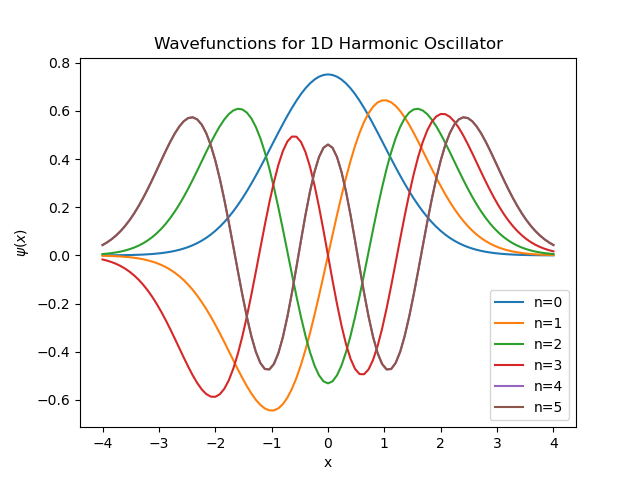
\includegraphics[width=0.8\textwidth]{./Problem_1/1d_harm_oscil.png} % Inserts the image, scaled to 80% of text width
    \caption{A plot of the 1-D harmonic oscillator wavefunctions calculated using the given equation and the code above. 
    Each energy level, $n$, is plotted using a different color shown in the legend.} % Caption for the figure
    \label{fig:example_figure} % Label for cross-referencing
\end{figure}
\clearpage
The plots make sense, and follow the traditional 1D harmonic oscillator wavefunctions.
\item 
  To calculate the N-dimensional harmonic oscillator wavefunctions at some radius $r$ for $D=2,3$, $\ell=0,1$, and $v=1$, I used the following code
  and relevant subroutines/functions:
\begin{verbatim}
!A program to calculate the N-dimensional radial wavefunction for the harmonic
!oscillator
program harmonic_oscillator_nd

    use numtype
    implicit none

    real(dp) :: wfunc(0:100), x, y
    integer :: nm, n, i
    real(dp) :: v

    nm = 5
    v = 1
    
     ! Test of the Laguerre polynomial function 
     ! do i = 0,100
     !   x = -2 + i * 1._dp/10
     !   write(17, *) x, Laguerre_P(3,0._dp,x) 
     ! end do

    do i = 0,200
        x = 0 + i * 4._dp/100
        ! Run for l = 0,1 , D = 2,3
        call wavefunction(nm,0,v,x,2,wfunc)
        write(02, *) x, wfunc(0:nm) 
        call wavefunction(nm,0,v,x,3,wfunc)
        write(03, *) x, wfunc(0:nm) 
        call wavefunction(nm,1,v,x,2,wfunc)
        write(12, *) x, wfunc(0:nm) 
        call wavefunction(nm,1,v,x,3,wfunc)
        write(13, *) x, wfunc(0:nm) 
    end do


     print *, 'Computing N-D Harmonic Oscillator functions ...'

    contains 
        ! This is a function to calculate the wavefunction from the Laguerre polynomials
        subroutine wavefunction(nm,l,v,r,D,lpoly)
  
          use numtype
          implicit none
          
          integer, intent(in) :: nm, l, D
          real(dp), intent(in) :: r, v
          real(dp), dimension(0:nm), intent(out) :: lpoly
          integer :: n
          real(dp) :: coeff

          do n = 0, nm 
            ! Multiply eaech Laguerre polynomial by the respective coefficient
            coeff = v**(0.25_dp)*(2*gamma(n+1._dp)/gamma(n+l+D/2._dp))**(0.5_dp)*exp(-v*r**2/2)*(v*r**2._dp)**(l/2._dp+(D-1)/4._dp)
            lpoly(n) = coeff*Laguerre_P(n,l+D/2._dp - 1,v*r**2)
          end do

        end subroutine wavefunction

        !This is a recursive function to calculate the Associated Laguerre polynomals
        recursive function Laguerre_P(n,a,x) result(s0)   
            use numtype
            implicit none

            integer, intent(in) :: n
            real(dp), intent(in) :: x, a
            real(dp) :: s0

            if(n < 0) then
                s0 = 0
            else if (n==0) then
                s0 = 1._dp
            else if (n==1) then
                s0 = 1 + a - x
            else 
                ! Calculation of the Laguerre polynomials for n>1
                s0 = ((2*n-1+a-x) * Laguerre_P(n-1,a,x) - (n-1+a) * Laguerre_P(n-2,a,x))/n
            end if    
    
        end function Laguerre_P

end program harmonic_oscillator_nd
\end{verbatim}

In this code, the recursive function `Laguerre P()' calculatees the Laguerre polynomial function for the recursion relation that we were given in class. 
The subroutine `wavefunction()' then calculates the coefficients including the gamma functions outside the given equation for the N-D wavefunction. These
coefficients are then multiplied by each Laguerre polynomial for each $n$. The plots for this code are shown below.
\begin{figure}[h!]
    \centering
    \subfigure(a){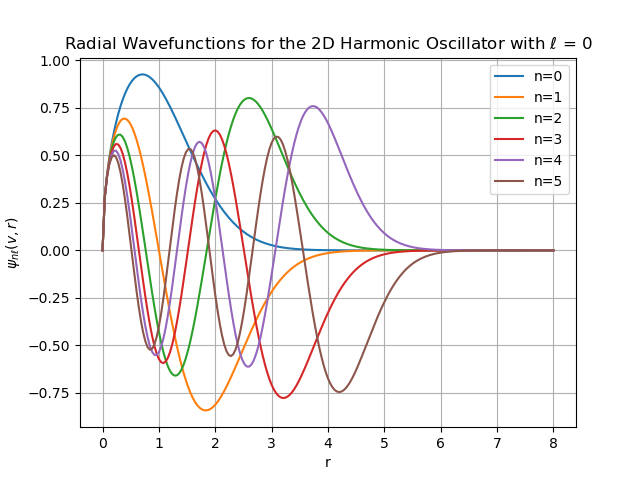
\includegraphics[width=0.4\textwidth]{./Problem_2/plots/Wf_0l_2-D.png}} 
    \subfigure(b){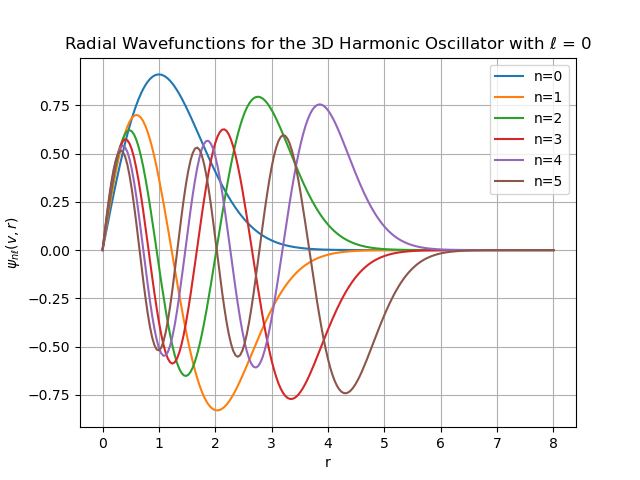
\includegraphics[width=0.4\textwidth]{./Problem_2/plots/Wf_0l_3-D.png}} 
    \subfigure(c){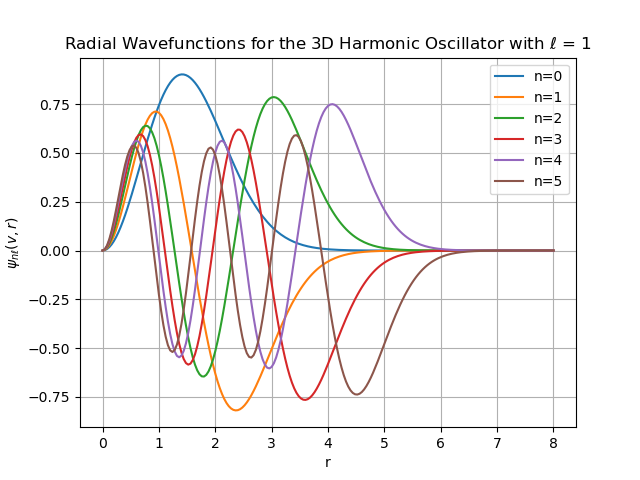
\includegraphics[width=0.4\textwidth]{./Problem_2/plots/Wf_1l_3-D.png}}
    \subfigure(d){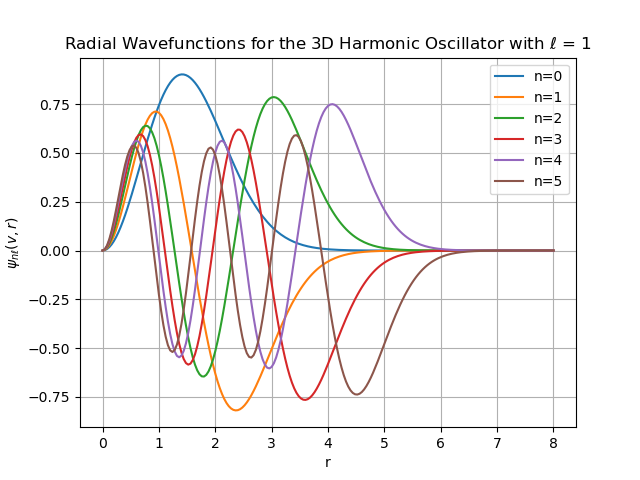
\includegraphics[width=0.4\textwidth]{./Problem_2/plots/Wf_1l_3-D.png}}
    \caption{(a) 2D harmonic oscillator radial wavefunction for $\ell=0$ (b) 3D harmonic oscillator radial wavefunction for $\ell=0$ (c) 2D harmonic oscillator radial wavefunction for $\ell=1$  (d) 3D harmonic oscillator radial wavefunction for $\ell=1$.  
    In each plot, the energy levels from $n=0,1,...5$ using different colors according to the legend. In each wavefunction, $v=1$.}
    \label{fig:foobar}
\end{figure}

These plots make sense since the wavefunction starts at 0 for $r=0$, but I worry there is some type error in combining integers and double precision floats
in my code. This is because there seems to be little difference in the plots for the change in angular momentum quantum number from 0 to 1. Generally, the 
overall structure of the wavefunctions makes sense for a particle in a 2D and 3D harmonic oscillator well.

\end{enumerate}

 
% --------------------------------------------------------------
%     You don't have to mess with anything below this line.
% --------------------------------------------------------------
 
\end{document}

